%!TEX root = ../thesis.tex
%*******************************************************************************
%*********************************** Sixth Chapter *****************************
%*******************************************************************************

\chapter{Application of CPACE model \label{cha:application}}  %Title of the Sixth Chapter

\ifpdf
    \graphicspath{{Chapter6/Figs/Raster/}{Chapter6/Figs/PDF/}{Chapter6/Figs/}}
\else
    \graphicspath{{Chapter6/Figs/Vector/}{Chapter6/Figs/}}
\fi
The CPACE model as described in Chapter~\ref{cha:cpace} is designed to allow for functional data which are observed dependently.
Most often this may be a spatial dependence between neighbouring trajectories although the framework discussed isn't reliant on this.
We have shown theoretically how we would reconstruct unobserved trajectories using our estimators. 
However, we are yet to highlight in practice the ability of such estimators and their reconstruction ability.
In the following chapter we present a series of simulated results designed to test the estimator capabilities, namely the ability to recover model hyper parameters. 
Following this we present the application of the CPACE model to the CESM-LE dataset, as discussed in Chapter~\ref{cha:data}, and contrast this against the traditional FPCA PACE model which doesn't utilise the spatial information of the data.

\section{Simulation Study \label{sec:sim_study}}
In the following section we present a simulation study based on the simulation study of \cite{yao_functional_2005}.
This simulation study was designed in \cite{yao_functional_2005} to showcase the implementation of sparse functional principal components analysis which are observed independently.
We will take this study as a base and then develop their generating procedure to allow for spatial dependency between functional observations.
We refer in the following to spatial dependency between functional observations because our main application of the CPACE model is the EO data, which naturally has spatial dependency.
However, this simulation study, and indeed the CPACE model can naturally be applied with different dependency between functional observations.

The simulation study consists of four scenarios; namely A, B, C, and D.
In each scenario the functional data are generated from the same mean and principal components.
We vary the spatial dependence between each scenario to show how the CPACE model with different spatial kernels can accommodate differing spatial structures.
We detail the exact specification for each scenario in its respective subsection.
First we describe the common underlying data generating process for the functional data.

\subsection{Data Generating Process \label{ssec:dgp_sim}}
We propose the simulations to be generated over temporal domain $\mathcal{T} \in \left[0, 10\right] \subset \mathbb{R}$.
The processes have mean $\mu\left(t\right) = t + \sin\left(t\right)$ and generated as in Equation \eqref{eqn:fpca_cpace} with $K=2$.
The eigenfunctions are given by: 
\begin{eqnarray}
	\phi_1\left(t\right) &=& -\frac{1}{\sqrt{5}}\cos\left(\frac{\pi t}{10}\right) \nonumber \\ 
	\phi_2\left(t\right) &=& -\frac{1}{\sqrt{5}}\sin\left(\frac{\pi t}{10}\right) \nonumber \\
\end{eqnarray}

Figure~\ref{fig:sim_mean} displays the mean function we use for the simulation, and Figure\ref{fig:sim_eig} highlights the variation from the mean that each eigenfunction contributes. As can be seen, the mean function used for the simulation has a clear upward trend and a periodic component. The first eigenfunction represent periodic variation at the start and end of the temporal domain, with the second eigenfunction giving variation in the middle of the temporal domain.

\begin{figure}
	\centering
	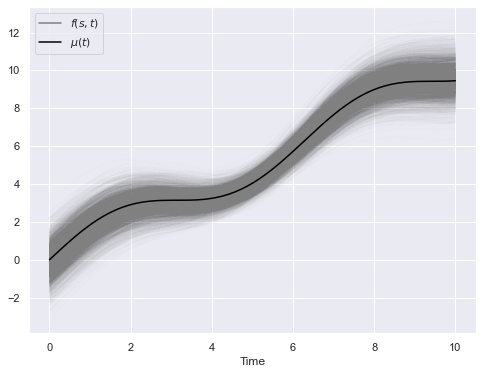
\includegraphics[width=\textwidth]{mean_sim}
	\caption{The mean function chosen for the simulation study over the temporal domain. We have illustrated example functional data simulated using this mean function in grey.}
	\label{fig:sim_mean}
\end{figure}

\begin{figure}
	\centering
	\begin{subfigure}[b]{0.45\textwidth}
		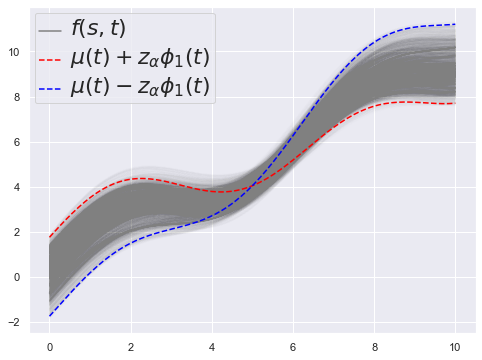
\includegraphics[width=\textwidth]{sim_eig_1}
		\caption{Variation from the mean function caused by the first eigenfunction.}
		\label{fig:sim_eig1}
	\end{subfigure}
	\hfill        
	\begin{subfigure}[b]{0.45\textwidth}
		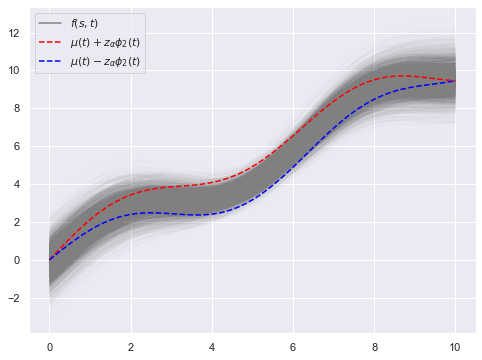
\includegraphics[width=\textwidth]{sim_eig_2}
		\caption{Variation from the mean function caused by the second eigenfunction.}
		\label{fig:sim_eig2}
	\end{subfigure}
	\caption{An example of the variation due to the two eigenfunctions from the mean function. We choose to highlight the variation with variance $4$ and $1$ respectively, as this is the kernel variance chosen for the simulation study. This choice is discussed below. Again we highlight example functional data generated from this setup in grey.}
\end{figure}

We propose to simulate observations on the spatial domain of $\mathcal{S} = \left[-5, 5\right] \times \left[-5, 5\right] \subset \mathbb{R}^2$.
Where each location $\ve{s} \in \mathcal{S}$ can give rise to a functional data generated by the above mean and principal components by Equation \eqref{eqn:fpca_cpace}.
In order to generate such data in practice we discretise the temporal domain to a fine grid by segmenting $\mathcal{T}$ into $128$ equal segments, and use the midpoints for generation of the functional data.
For each functional observation we suppose, as in \citep{yao_functional_2005} and our setup in Chapter \ref{cha:Into}, that we do not observe the full true function $\mathcal{X}\left(\ve{s}, t\right)$ but we sparsely observe a noisy version of it.
For all the simulations we suppose our noise variance is $\sigma^2_\epsilon = 0.25$. 
We suppose the sparsity of observations is between $5\%$ and $10\%$ of our full $128$ temporal grid.
That is our number observation points are chosen uniformly from $\left[6, 7, \cdots, 11, 12\right]$.
The observation points are sampled randomly from the full discretized grid over $\mathcal{T}$.
This is a slight deviation from the simulation study in \citep{yao_functional_2005} but lies closer to reality for EO data which is often observed at regular grid intervals.
Figure~\ref{fig:sim_example} highlights an example of the sparsity and observation error described above.

\begin{figure}
	\centering
	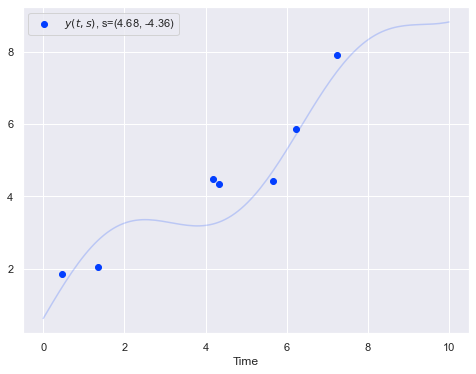
\includegraphics[width=\textwidth]{sim_ex}
	\caption{An example functional data with observation points. This example is taken from Scenario A and highlights the sparsity of observation as well as the impact of the noise variance on observations.}
	\label{fig:sim_example}
\end{figure}

For the spatial domain we consider $\mathcal{S} = \left[-5, 5\right] \times \left[-5, 5\right] \subset \mathbb{R}^2$.
Again in practice we discretize this into $64$ equally spaced segments across the first domain, and $48$ equally spaced segments across the second domain.
Again we take the midpoints as our discretized sampling locations.
This gives in total $64 \times 48$ possible sampling locations for our simulation study.
We take half of our sampling locations as observed data, that is used to estimate the parameters of the CPACE model.
Namely, the spatial kernel hyper-parameters and eigen decomposition parameters.
As we only observe each functional datum sparsely this corresponds to a training dataset of approximately $3.75\%$ of the total discretized points of simulation.

As stated above, to simulate spatially dependent functional data we must simulate a realisation of our spatial covariance process $\zeta_i(\ve{s})$ for $i=1,2$. 
The particular form of this process will change in each scenario but we keep the variance of these processes consistent to align closely with the study in \citep{yao_functional_2005}.
That is we set the variance of $\zeta_1$ to be $4$ and $\zeta_2$ to be $1$, which corresponds to $\lambda_1 = 4$ and $\lambda_2=1$ from Chapter~\ref{cha:cpace}.

Finally, we simulate $50$ replications using the above data generating procedure to produce our scenario dataset.
For each simulation of each scenario we will evaluate various versions of the CPACE model against the standard FPCA model which doesn't take into account the spatial correlation between functional observations.
We discuss the evaluation of our models against these simulated data in the following section. 

\subsection{Evaluation metrics \label{ssec:eval_metrics}}
To evaluate the performance of our model we consider two standard metrics; the mean square error, mean absolute error.
The first two are standard evaluation metrics for a regression based model but for clarity the mean square error and mean absolute error for prediction $\hat{\mathcal{X}}$ against unobserved functional data $\mathcal{X}$ is given by:

\begin{eqnarray}
	MSE = \frac{1}{50} \sum_{i=1}^{50} \int \int \left( \mathcal{X}(\ve{s}, t) - \mathcal{X}(\ve{s}, t) \right)^2 d\ve{s} dt \nonumber \\
	MAE = \frac{1}{50} \sum_{i=1}^{50} \int \int \left| \mathcal{X}(\ve{s}, t) - \mathcal{X}(\ve{s}, t) \right| d\ve{s} dt \nonumber
\end{eqnarray}
In practice, we evaluate these on the discrete simulation grid and use numerical integration to approximate these metrics.

For our simulation study we have three distinct sets of data to evaluate performance against.
The training data set, which comprises solely on the location and time points for which we observe our noisy dataset.
The validation dataset which comprises of the locations of where we observe our noisy data, but including unobserved time points. 
Finally, the test dataset which comprises of completely unseen locations and time points.
Comparing the performance of the CPACE model against the standard FPCA model against each dataset should highlight how well our CPACE model performs under the three separate conditions.
Greater performance on the test dataset is most preferable as it shines insight functions at unobserved locations.
To place back in the context of EO data, this could be useful to interpolate data where it is not possible to get physical observations.
The validation dataset highlights the ability of the model to recover observations from a possibly malfunctioning data source which leads to partial observations at a particular location.
The training dataset is typically the easiest to achieve good performance on and is most suitable for evaluation of the model at its ability to overcome observation error.

In this study we will examine the performance of the CPACE model with four different spatial kernels. Three of which correspond to stationary kernels, and one which is designed to model non-stationary spatial dependence. We detail them below: 

\subsection{Spatial Kernels  \label{ssec:spatial_kern}}
We choose four kernels to examine. The first of which, Section~\ref{sssec:white_kern}, corresponds to the kernel with no spatial dependence, and is chosen to highlight the ability of the CPACE model to recreate the PACE model. The next two, Sections~\ref{sssec:matern_one},~\ref{sssec:matern_three} correspond to common spatial kernels, one of which is used in the SPACE model, \citep{liu_functional_2017}. These highlight the CPACE model's ability to capture quite simplistic spatial correlation structures. The final, Section~\ref{sssec:gibbs}, is a less commonly used kernel which capture non-stationarity in the spatial dependence. This kernel is chosen to highlight that the CPACE model can effectively be used in cases of highly complex spatial dependence. As in Chapter~\ref{cha:background} we refer the reader to \cite{cressie_statistics_2011} for a more in depth discussion of various covariance structures in spatial statistics.

\subsubsection{White Kernel \label{sssec:white_kern}}
The White, or Independent kernel, is the simplifying assumption which reverts the CPACE model to the standard PACE model. That is it defines the covariance between $\vesub{s}{i}$ and $\vesub{s}{j}$ as follows:

\begin{equation}
	\zeta_k\left(\vesub{s}{i}, \vesub{s}{j}\right) = \lambda_k\delta_{ij}
\end{equation}
where 
\begin{equation*}
\delta_{ij} = \begin{cases}
	1 & \text{if } \vesub{s}{i} = \vesub{s}{j}, \\
	0 & \text{otherwise}
\end{cases} 
\end{equation*}

This kernel places zero correlation between functional data at differing spatial locations, and a variance of $\lambda_k$ between functional observations at the same locations.
Note that this corresponds to the full cross-correlation of $\mathcal{X}\left(\vesub{s}{i}, t \right)$ and  $\mathcal{X}\left(\vesub{s}{j}, t \right)$ under our initial example given by Equation~\ref{eqn:principal_comp_uncorr} in Chapter~\ref{cha:background}.
The added distinction that we are now using $\ve{s}$ to indicate spatial location rather than an simple index.
Figure~\ref{fig:ex_white} displays the covariance matrix given by this kernel over our spatial domain $\mathcal{S}$. 

\begin{figure}
	\centering
	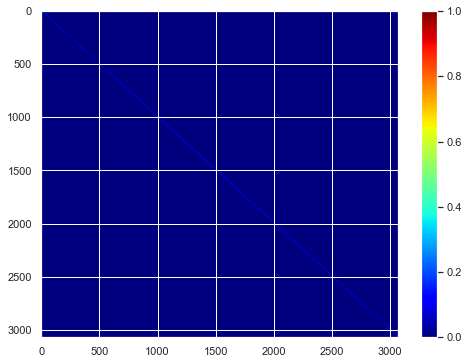
\includegraphics[width=\textwidth]{ex_white}
	\caption{The covariance between all points in out spatial domain $\mathcal{S}$ with the above covariance function. Each index on the axis corresponds to a point $\ve{s}_i$ in $\mathcal{S}$ in our discretised grid. Notice it is one on the diagonal, and zero elsewhere.}
	\label{fig:ex_whiite}
\end{figure}

As such the use of this kernel in the CPACE model will result in essentially a differing view of the PACE model under which there is assumed no spatial correlation.

\subsubsection{Mat\'ern One Half Kernel \label{sssec:matern_one}}
The Mat\'ern kernel is a standard in the spatial statistics literature, \cite{cressie_statistics_2011}.
This is an specific example of the general form by setting $\nu=0.5$. 
When setting this shape parameter it leads to a simple closed form, given below:

\begin{equation}
	\zeta_k\left(\vesub{s}{i}, \vesub{s}{j}\right) = \lambda_k \exp \left( -\frac{d}{\rho} \right)
\end{equation}
where $d = \lVert \vesub{s}{i} - \vesub{s}{j} \rVert$.
This kernel is often used due to its simplicity to compute while it maintains good ability to capture stationary covariances.
We use the Euclidean distance for the calculation of $d$ which makes this kernel isotropic.
The length scale parameter, $\rho$, is used to capture the correlation over differing spatial scales.
In the CPACE model we treat $\rho$ as a hyper parameter to estimate.
This estimation procedure is described in Chapter\ref{cha:cpace} with more implementation details in Chapter~\ref{cha:implementation}.
Figure~\ref{fig:ex_mat_1} shows the covariance on our spatial domain $S$ with length scale, $\rho$,  and variance $lambda_k$ equal to $1$ .


\begin{figure}
	\centering
	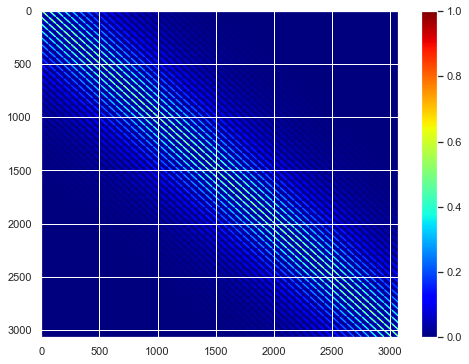
\includegraphics[width=\textwidth]{ex_mat_1}
	\caption{The covariance between all points in out spatial domain $\mathcal{S}$ with the above covariance function. Each index on the axis corresponds to a point $\ve{s}_i$ in $\mathcal{S}$ in our discretised grid.}
	\label{fig:ex_mat_1}
\end{figure}

The use of this model is akin to the SPACE model, \citep{liu_functional_2017}.
However in the CPACE model the estimation procedure for hyper parameters is different.

\subsubsection{Mat\'ern Three Halves Kernel \label{sssec:matern_three}}
Similar to the Mat\'ern One Half kernel, Section~\ref{sssec:matern_one}, this is another specific example of the general Mat\'ern covariance kernel.
This time we set the shape parameter $\nu$ to $3.5$.
This leads to the specific closed form of the covariance kernel given below:

\begin{equation}
	\zeta_k \left(\vesub{s}{i}, \vesub{s}{j}\right) = \lambda_k \left(1 + \frac{\sqrt{3}d}{\rho} \right)\exp \left(\frac{- \sqrt{3}d}{\rho} \right)
\end{equation}
where again $d$ is the euclidean distance between $\vesub{s}{i}$ and $\vesub{s}{j}$ given by $d = \lVert \vesub{s}{i} - \vesub{s}{j} \rVert$. 
Again, this is a stationary kernel, that is the covariance between two points depends only on the spatial distance between points and not their location.
The length scale parameter, $\rho$, is used to capture the correlation over differing spatial scales. 
In the CPACE model we treat it as a hyper parameter to estimate.
Figure~\ref{fig:ex_mat_3} shows an example covariance structure over out spatial domain $\mathcal{S}$ for the simulation study.
We note that comparing this to Figure~\ref{fig:ex_mat_1} that the covariance model is naturally smoother that the Mat\'ern One Half kernel and in some sense is designed to model smoother variation over the domain.

\begin{figure}
	\centering
	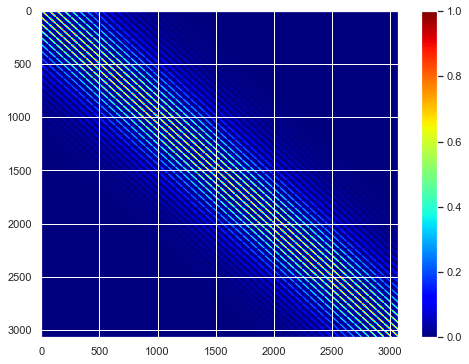
\includegraphics[width=\textwidth]{ex_mat_3}
	\caption{The covariance between all points in out spatial domain $\mathcal{S}$ with the above covariance function. Each index on the axis corresponds to a point $\ve{s}_i$ in $\mathcal{S}$ in our discretised grid.}
	\label{fig:ex_mat_3}
\end{figure}

Again, the use of this model is akin to the SPACE model, \citep{liu_functional_2017}.
However in the CPACE model the estimation procedure for hyper parameters is different.

\subsubsection{Gibbs Kernel \label{sssec:gibbs}}
All the above kernels are stationary.
Stationary kernels have been well studied due to the relative ease of estimation of kernel hyper parameters.
However, they are often too simplistic as many real world data sets exhibit some form of non-stationarity.
We consider the Gibbs kernel, named after the Gibbs who authored the thesis which first described this kernel, \citep{gibbs_bayesian_nodate}, in our simulation study as a non-stationary kernel which can account for more complex spatial dependence.
The form of the kernel is given succinctly by \citeauthor{paciorek_spatial_2006}, \citep{paciorek_spatial_2006}, for one dimensional input. 

\begin{equation}
	\zeta_k\left(s_{i}, s_{j}\right) = \lambda_k \sum_{q=1}^{Q} \sqrt{\frac{2l_q(s_i)l_q(s_j)}{l_q(s_i)^2 + l_q(s_j)^2}} \exp \left(-\frac{\left(s_i - s_j\right)^2}{l_q(s_i)^2 + l_q(s_j)^2}\right)
\end{equation}

This can be simply extended to two, as in our simulation case, or more dimensions by having a Gibbs kernel on each dimension of the input and combining by simply multiplying them together.
This remains a valid positive definite kernel as the product of two or more positive definite kernels remains positive definite. 
In this Gibbs kernel we have multiple components, referenced by $Q$ total components.
Each component has its separate length scale model $l_q(s)$ which controls the length scale parameters at each point in the domain.
In principal these length scale models can be arbitrary positive functions, and the Gibbs kernel remains valid.

Figure~\ref{fig:ex_gibbs} gives an example covariance function from the Gibbs kernel.
As can be seen, the covariance structure changes over the domain, highlighting the non-stationarity of the Gibbs model.
This can allow for much more complex spatial structures.
Here we have restricted the kernel to two components, and use as in Scenario D, the lengthscale model given by:
\begin{eqnarray}
	l_1(s) &=& \frac{1}{1 + \exp(-s)} \nonumber \\
	l_2(s) &=& \frac{1}{1 +  \exp(s)} \nonumber \\
\end{eqnarray}
For example, locations in the middle of the domain $\mathcal{S}$, are less correlated to immediate neighbours than the locations on the fringes of the domain.
This has been induced by the choice of the lengh scale models above.
In out simulation study, we treat these as hyper parameters to be estimated from the observed data.
The way in which we do so will be discussed in greater detail in Section~\ref{sec:sim_D} and in Chapter~\ref{cha:implementation}.

\begin{figure}
	\centering
	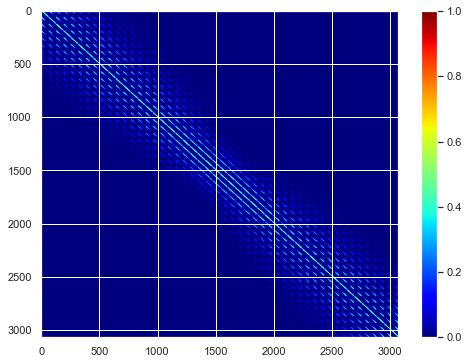
\includegraphics[width=\textwidth]{ex_gibbs}
	\caption{The covariance between all points in out spatial domain $\mathcal{S}$ with the above covariance function. Each index on the axis corresponds to a point $\ve{s}_i$ in $\mathcal{S}$ in our discretised grid.}
	\label{fig:ex_gibbs}
\end{figure}

Now we discuss the specific results of using the various kernels in our simulation studies. 



\section{Scenario A - Independent Functional Data \label{sec:sim_A}}
Our first simulation scenario considers the basic case when there is no spatial dependence between functional data.
This corresponds to the case that for each component we simulate data using a the White kernel, as described above.
As stated in Section~\ref{ssec:dgp_sim}, we consider $50$ replications using the White kernel with the aforementioned eigenfunctions with respective variance of $4$ and $1$. 
We consider $5$ models, the first being the standard PACE model as implemented in \citep{yao_functional_2005}.
This is our base model, and is referred to as \verb*|fpca| in the following tables and graphs. 
The second model we consider our CPACE model, using $5$ components, each with an independent White kernel.
This model is estimated under our framework of the CPACE model, and as such the kernel variances are initially estimated using the PACE methodology but additional refinement of the estimates is done through the CPACE framework.
This will be referred to as the \verb*|fpca_gp| model in the following metrics and graphs.
The third and fourth models are similar.
They correspond to the using the Mat\'ern One Half and Mat\'ern Three Halves kernels as spatial kernels in the CPACE model respectively.
Again, we use the CPACE framework to refine the noise and variance estimation, but in addition use the CPACE framework to estimate each kernels hyper parameter, $\rho_k$.
We refer to these models as \verb*|matern_one| and \verb*|matern _hree| respectively.
Finally the last model corresponds to using the Gibbs kernel for each components spatial kernel in the CPACE model.
We use $Q=5$ components for each Gibbs kernel.
The Gibbs kernel has length scale models.
For our simulation study we assume we can approximate the true length scale functions using a neural network.
This allows the model to be flexible to capture many different functions without having to be too specific in the setup of the model.
We use a standard multi-layer perceptron network with two layers.
Each length scale model has the same architecture of two fully connected hidden dense layers with $32$ neurons in each layer.
We use an rectified linear unit activation for the hidden layers, and a final activation which maps the length scale produced between $0.0001$ and $1$.
This is to ensure the length scales remain positive and bounded within a sensible value.
Under the CPACE model framework the parameters to each length scale model are estimated, along with the standard variance and noise variance estimation.
We refer to this model as \verb*|gibbs| in the following.

Running $50$ simulations, we first display, in Table~\ref{tab:train_A}he training metrics of the models, both the $MSE$ and the $MAE$ with their respective variance for the training observations from each simulation. 
We note here that, expectedly, the models which assume no spatial dependency do best on the training data.
Quiite simply, this is because the model is closest to the data generating procedure.
However, it is interesting to note that on observed training data all the models results with the CPACE framework are on a similar order of magnitude as that of the PACE model.
This is encouraging as suggest, that we don't loose anything by considering a more complex model, as the CPACE framework can adapt to independently observed data as the kernel parameters are estimated such that the kernel becomes close to the White kernel.

\begin{table}
	\caption[Simulation results for Scenario A on training data]{Simulation results for the models ability to estimate the functional values at points of observation. Bold indicates best in class.}
	\centering
	\label{tab:train_A}
	\begin{tabular}{lcc}
		\toprule
		\textbf{Model} & \textbf{MSE} & \textbf{MAE} \\
		\midrule
		\verb*|pace| & 0.0502 (0.0015) & 0.1771 (0.0026) \\
		\verb*|fpca_gp| & \textbf{0.0499 (0.0014)} & \textbf{0.1766 (0.0025)} \\
		\verb*|matern_one| & 0.0508 (0.0014) & 0.1782 (0.0025) \\
		\verb*|matern_three| & 0.0523 (0.0042) & 0.1805 (0.0069) \\
		\verb*|gibbs| & 0.0685 (0.0042) & 0.2052 (0.0115)\\
		\bottomrule
	\end{tabular}
\end{table}

Next we consider the metrics for reconstruction of the functional data across all observed locations.
This is akin to the combination of the validation and the training data sets as described above.
Table~\ref{tab:val_A} shows the metrics on these data points.

\begin{table}
	\caption[Simulation results for Scenario A on validation data]{Simulation results for the models ability to estimate the functional data at locations of observation across the whole temporal domain. Bold indicates best in class.}
	\centering
	\label{tab:val_A}
	\begin{tabular}{lcc}
		\toprule
		\textbf{Model} & \textbf{MSE} & \textbf{MAE} \\
		\midrule
		\verb*|pace| & 0.5641 (0.0168) & 1.8707	(0.0279) \\
		\verb*|fpca_gp| & \textbf{0.5609 (0.0158)} & \textbf{1.8659 (0.0269)} \\
		\verb*|matern_one| & 0.5722	(0.0163) & 1.8845 (0.0264) \\
		\verb*|matern_three| & 0.5901 (0.0482) & 1.9109	(0.0744) \\
		\verb*|gibbs| & 0.7782 (0.1067) & 2.1510 (0.1224)\\
		\bottomrule
	\end{tabular}
\end{table}

We can see clearly, the same pattern as from the training metrics. 
Again, the \verb*|fpca_gp| model is our best in terms of reconstruction ability.
Figure~\ref{fig:val_ex_A} highlights a single example of such reconstruction.
It can be seen that not only the \verb*|fpca_gp| model captures the full unobserved functional data well and it does so well with confidence using the variance the follows from the CPACE framework.
It is easy to see that the \verb*|gibbs| model fails to capture as completely the functional data, possibly due to error in estimation of the  length scale models.
This may be because we have assumed a complex form of the length scale models in the \verb*|gibbs| model and the estimation procedure for them has failed to converge appropriately to the simple form they take in this scenario.

 \begin{figure}
 	\centering
 	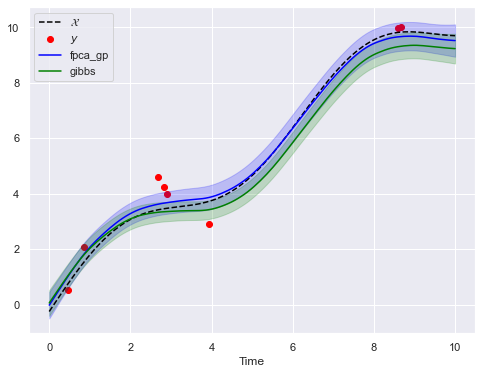
\includegraphics[width=\textwidth]{ex_val_A}
 	\caption{An indicative example of the CPACE model performance on reconstruction of functional data where noisy observations have been made.}
 	\label{fig:val_ex_A}
 \end{figure}

\section{Scenario B - Stationary Functional Data \label{sec:sim_B}}

\section{Scenario C - Complex Stationary Functional Data \label{sec:sim_C}}

\section{Scenario D - Non-Stationary Functional Data \label{sec:sim_D}}







